\documentclass[12pt]{article}
\usepackage[utf8]{inputenc}
\usepackage[T1]{fontenc}
\usepackage{amsmath,amsfonts,amssymb}
\usepackage{graphicx}
\usepackage{a4wide}

\usepackage{natbib}
\usepackage{hyperref} 
\usepackage{float}


\hypersetup{
    colorlinks=true,
    linkcolor=blue,
    citecolor=blue,
    urlcolor=blue
}

\bibliographystyle{apalike}



\title{Leveraging Adaptive Loss Scaling and Embeddings for Label Correction}
\author{Kirill Pupkov, Igor Ignashin, Aleksandr Beznosikov}
\date{2025}
\begin{document}
\maketitle

\begin{abstract}

    In machine learning, numerous challenges can degrade model performance, including noisy features and incorrect labeling in the training data. Various approaches exist to mitigate these issues, such as Adaptive Loss Scaling. In this paper, we propose an improvement to this approach by incorporating a label correction mechanism. Our method replaces the labels of high-loss samples with those of their nearest neighbors in the embedding space. We demonstrate the effectiveness of our approach on the MNIST dataset with a fraction of noisy labels.

\end{abstract}

\section{Introduction}

Machine learning models are often applied under the assumption that training data are correctly labeled and accurately represent the true data distribution. However, in practice, training sets often contain noisy labels, negatively affecting model performance. Various approaches have been proposed in the literature to address this issue.

One common strategy involves filtering out objects whose labels do not match the labels of their neighbors. For instance, \textit{Deep $k$-Nearest Neighbors filtering} \citep{bahri2020deepknn} uses a preliminary trained model to identify incorrectly labeled examples by comparing an object's label with those of its neighbors. This approach effectively removes mislabeled samples, improving the accuracy of the final model and often outperforming more complex robust training methods.

Another family of approaches focuses on reweighting training examples. Some methods utilize meta-learning to learn these weights \citep{ren2018learning}, while others use specialized networks to determine them \citep{jiang2018mentornet}. Recent work \citep{also} discusses how the task of assigning weights can be formulated as a min-max optimization problem and proposes a method for solving it using the ALSO optimizer.

In this paper, we propose a method to leverage the learned weights from the ALSO optimizer to progressively identify and relabel mislabeled training examples, improving model accuracy. Following the approach of \citet{bahri2020deepknn}, we utilize object embeddings to determine the correct labels.

The main contributions of our paper include:
\begin{itemize}
    \item \textbf{A new method for label correction.} We introduce a novel approach leveraging recent advances in robust learning and embedding-based methods.
    \item \textbf{Empirical evaluation.} We extensively evaluate our approach and compare it against state-of-the-art methods, demonstrating superior performance.
\end{itemize}

Formally, let \(\mathcal{D} = \{(x_i, y_i)\}_{i=1}^{n}\) be a clean dataset where \(y_i\) is the true label for the object \(x_i\). We observe a noisy training set \(\tilde{\mathcal{D}} = \{(x_i, \tilde{y}_i)\}_{i=1}^{n}\), where \(\tilde{y}_i\) may differ from \(y_i\).

We typically optimize the following objective:
\begin{equation}
    \min_{\theta \in \Theta} \left\{
        \frac{1}{n}\sum_{i=1}^{n} f_i(\theta) + \frac{\tau}{2}\|\theta\|_2^2
    \right\},
\end{equation}
where \(f_i(\theta) := L(q(\theta, x_i), \tilde{y}_i)\) is the loss function computed using the noisy labels, \(\tau > 0\) is a regularization parameter, and \(\frac{\tau}{2}\|\theta\|_2^2\) is the regularization term to prevent overfitting. However, as previously mentioned, optimizing this objective directly might lead to memorization of incorrect labels and therefore poor performance.

To address this, \citet{also} propose the following reformulation:

\begin{equation}
    \max_{\pi \in \Delta_{n-1}} \min_{\theta \in \Theta}
    \left\{
        \sum_{i=1}^{n}\pi_i f_i(\theta)
        + \frac{\tau}{2}\|\theta\|_2^2
        - \tau\text{KL}[\pi\|\hat{\pi}]
    \right\},
\end{equation}
where \(\tau > 0\) is the regularization parameter (temperature), \(\text{KL}[\cdot\|\cdot]\) denotes the KL-divergence between two distributions, and \(\hat{\pi}\) is a prior distribution of weights from \(\Delta_{n-1}\). A simple baseline choice for \(\hat{\pi}\) is the uniform distribution \(\hat{\pi} = \mathcal{U}(\mathbf{1}, n)\). This formulation encourages higher weights for samples that are more difficult to classify correctly, helping identify potentially mislabeled data.

In later sections, we demonstrate how to leverage iteratively computed weights \(\pi_i\) to effectively identify and correct mislabeled data points.

\section{Experiments}

\subsection{Data}

To evaluate the effectiveness of our algorithm, we conducted experiments using the MNIST dataset \citep{deng2012mnist}, which consists of 60,000 28$\times$28 grayscale images of handwritten digits. To simulate label noise we randomly selected a proportion $p$ of samples from the training set and assigned them incorrect labels. We then compared our algorithm against baseline methods across various noise levels to assess its performance.

\subsection{Evaluation Metrics}

We evaluated the performance of our approach using multiple metrics:

\begin{enumerate}
    \item \textbf{Precision}: The fraction of samples identified as mislabeled that were actually mislabeled
    \item \textbf{Recall}: The fraction of truly mislabeled samples that were successfully identified by the algorithm
    \item \textbf{Test Accuracy}: The classification accuracy achieved on the clean, uncorrupted test set after training with our noise-handling approach
\end{enumerate}

All experiments were run 5 times with different random seeds, and we report 95\% confidence intervals in our plots to account for variability.

\subsection{Baseline}

\subsection{Results}

\begin{figure}[H]
    \centering
    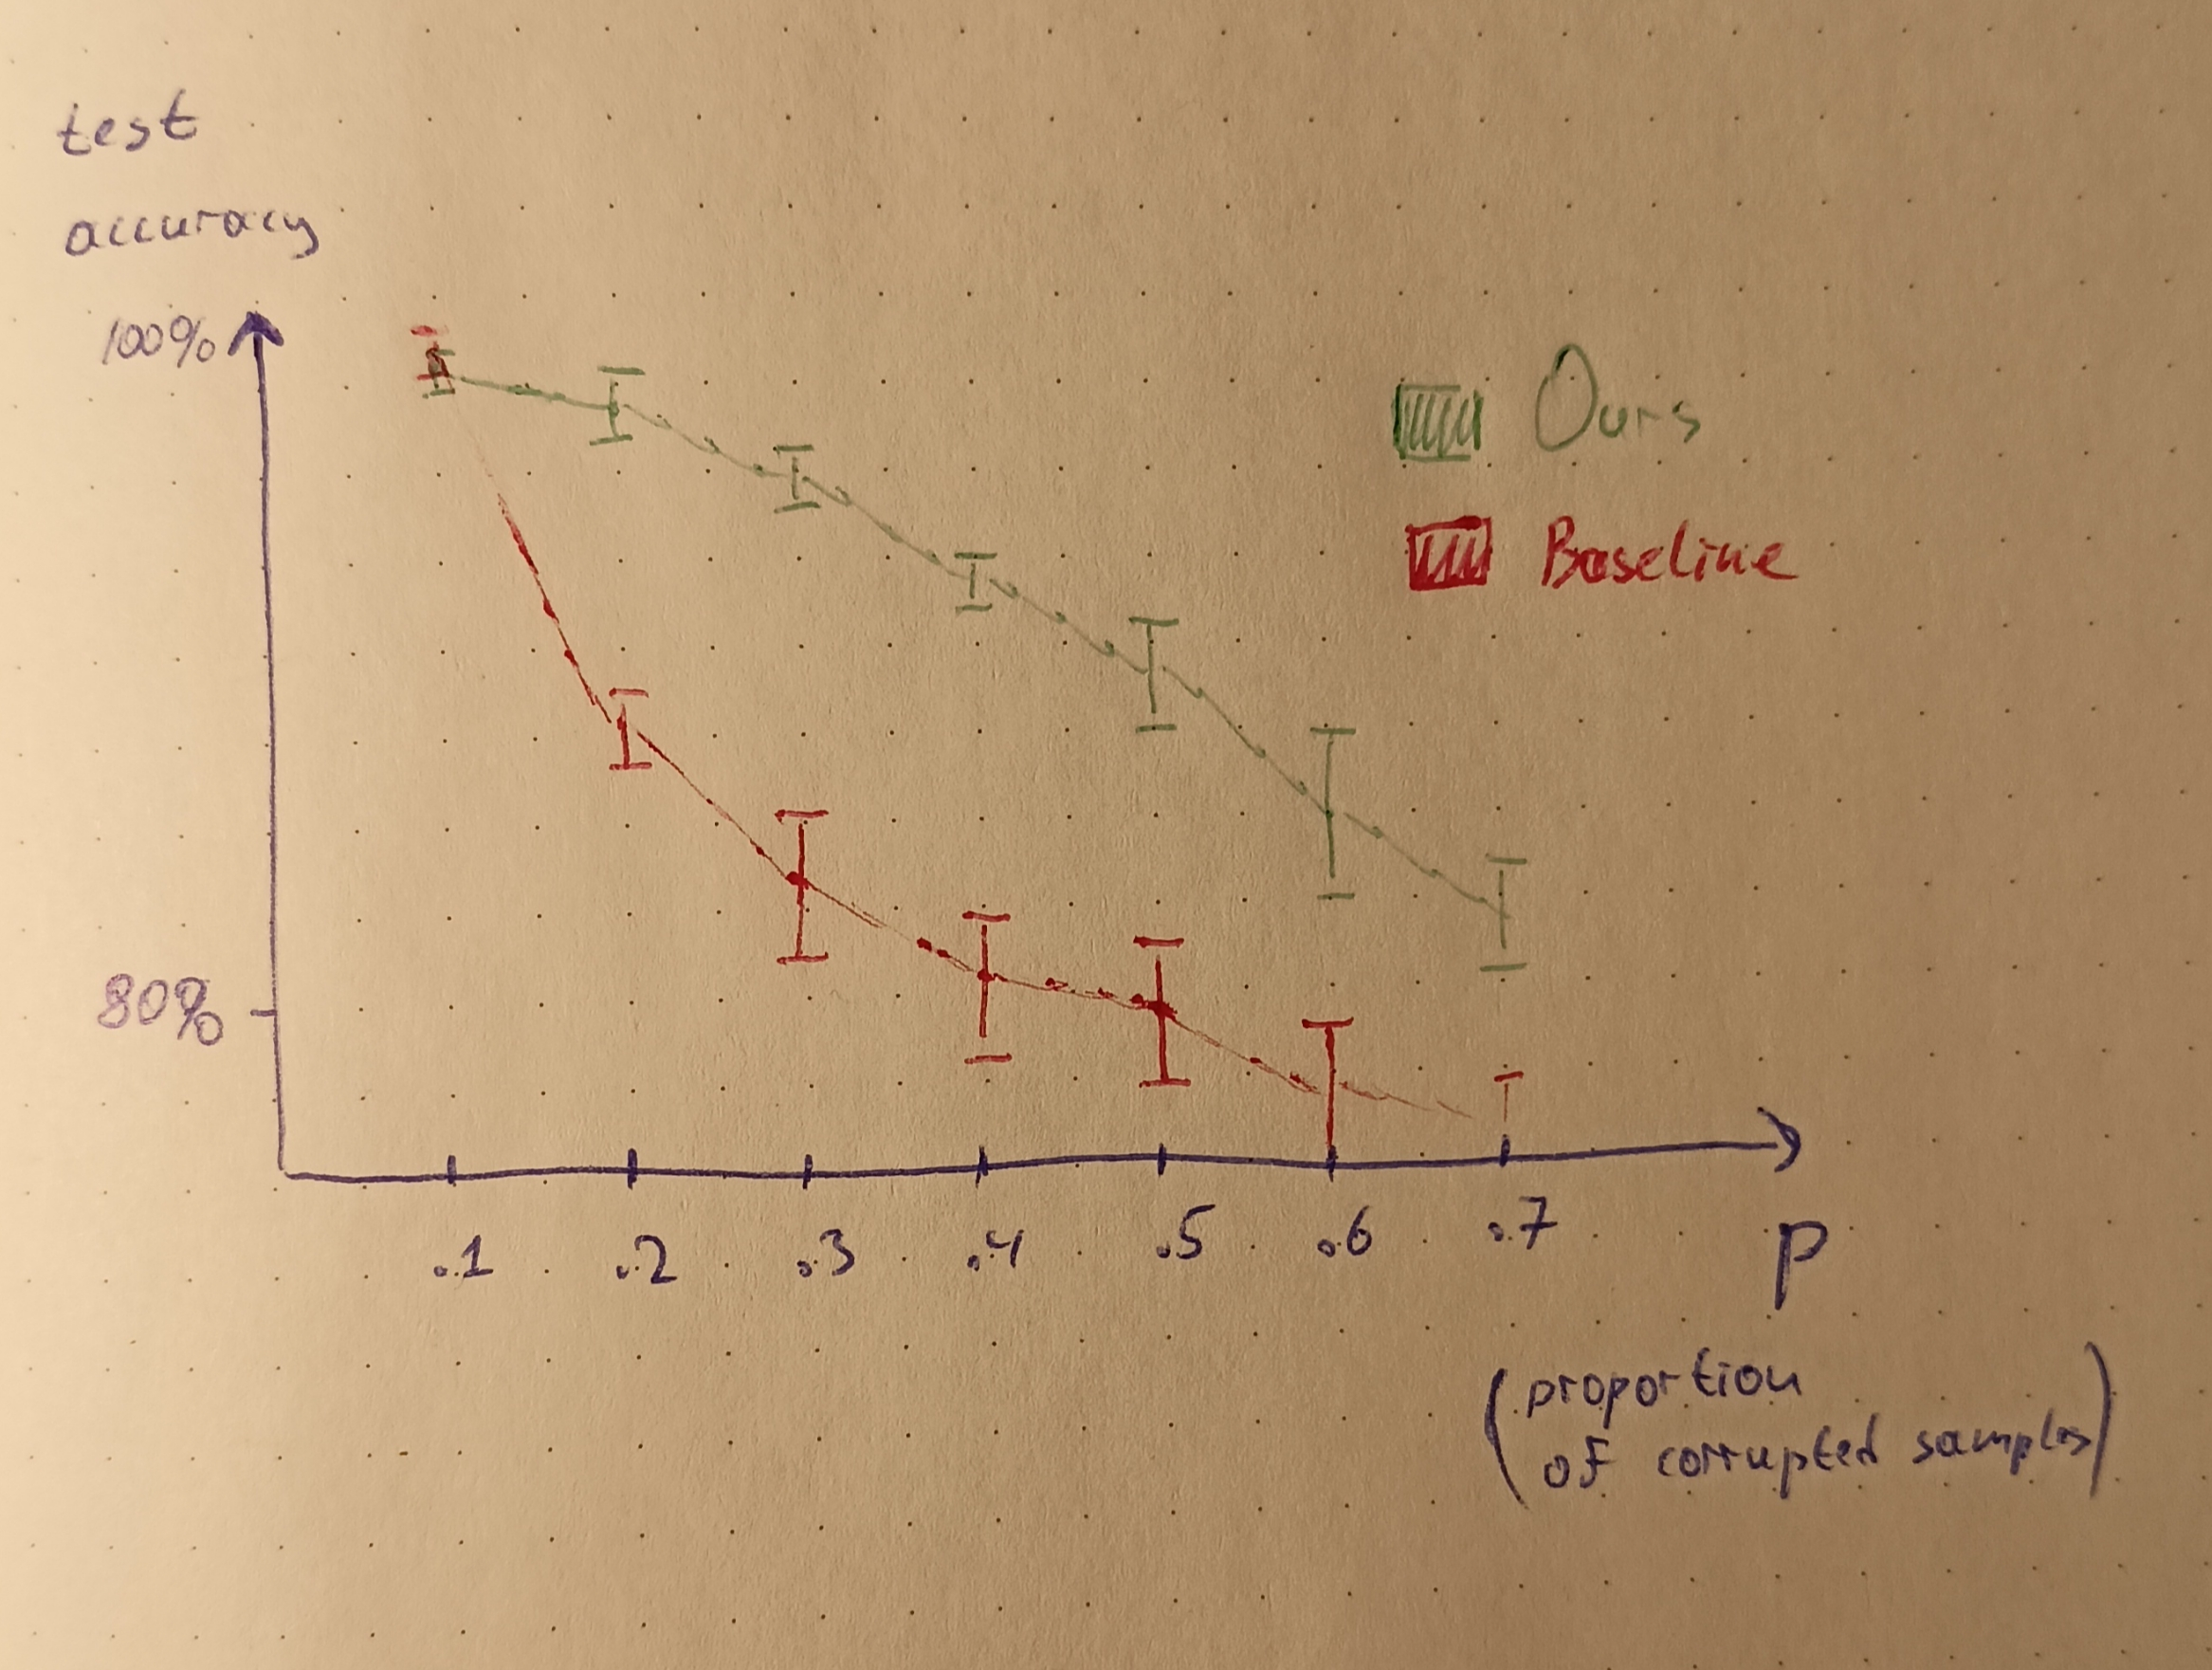
\includegraphics[width=0.9\linewidth]{figures/example_plot.jpg}
    \caption{Performance comparison of our proposed method versus baseline approach across different noise levels. Bars represent 95\% confidence intervals over 5 runs.}
    \label{fig:noise_detection}
\end{figure}

As shown in Figure~\ref{fig:noise_detection}, our method consistently outperforms the baseline approach in identifying mislabeled examples, particularly as the noise level increases.








\bibliography{references}

\end{document}